\documentclass[18pt,aspectratio=149]{beamer}
\usepackage[]{bookmark}
\usepackage[utf8]{inputenc}
\usepackage{amsmath}
\usepackage{amsfonts}
\usepackage{amssymb}
\usepackage{tikz}
\usepackage{xcolor}
\usepackage[dutch]{babel}
\usepackage{sansmathaccent}
\usepackage{graphicx}
\usepackage{pgfplots}

\usepackage[style=authoryear,backend=biber]{biblatex}


\DeclareBibliographyDriver{article}{%
    \printnames{author}%
    \setunit{\addspace}%
    \printfield{year}%
    \setunit{\addspace}%
    \printfield{title}%
    \finentry}

\DeclareBibliographyDriver{misc}{%
    \printnames{author}%
    \setunit{\addspace}%
    \printfield{year}%
    \setunit{\addspace}%
    \printfield{title}%
    \finentry}

\addbibresource{bibliography3.bib} 
\pdfmapfile{+sansmathaccent.map}

\title{RMC voor lineaire ODEs}
\author{Isidoor Pinillo Esquivel }
\usetheme{Madrid}

\date{}

\begin{document}

% 1 min
\begin{frame}
    \titlepage
\end{frame}

\section{Introductie}
% 2 min
\begin{frame}
    \frametitle{Introductie}
    \begin{equation}
        y_{t} = A(t)y(t)
        .
    \end{equation}
    \action<+->{}
    Euler:
    \begin{alignat}{2}
        \action<+->{\frac{\tilde{y}(t_{k}+\Delta t)-\tilde{y}(t_{k})}{\Delta t} & = & A(t_{k})                        & \tilde{y}(t_{k}) \\
        }
        \action<+->{\tilde{y}(t_{k+1})                                          & = & (I+\Delta t A(t_{k}))           & \tilde{y}(t_{k}) \\
        t_{k+1}                                                                 & = & t_{k}+\Delta            t     }                    \\
        \action<+->{Y(T_{k+1})                                                  & = & (I+\Delta t A(T_{k+1}))         & Y(T_{k})         \\
        T_{k+1}                                                                 & = & T_{k} + \text{Exp}(\Delta t)
        }
    \end{alignat}
    \action<+->{
        \begin{equation}
            y(T_{k})=E[Y(T_{k})].
        \end{equation}
    }

\end{frame}

% 1 min
\begin{frame}
    \frametitle{Overzicht}
    \tableofcontents
\end{frame}

% 2 min
% Ik heb 2 jaar terug een paper gelezen waardat men een WoS algoritme
% voorstellen voor elliptisch PDEs met plaats afhankelijke coëfficiënten.
% Het grote voordeel van dit algoritme is dat het unbiased is en 
% werkt voor complexe domeinen. Ik ben geïntereseerd om dit probleem 
% te veralgemenen met tijd afhankelijkheid. Er zijn papers die 
% WoS uitbreiden via een Euler scheme in de tijd maar deze zijn biased.
% Ik ben dan eerst gaan kijken hoe dat we Euler unbiased kunnen maken.

\section{Motivatie}
\begin{frame}
    \frametitle{Motivatie}
    Veralgemenen van WoS algoritme van (\cite{sawhney_grid-free_2022})
    naar tijd
    \vspace{-0.25cm}
    \begin{figure}[h!]
        \centering
        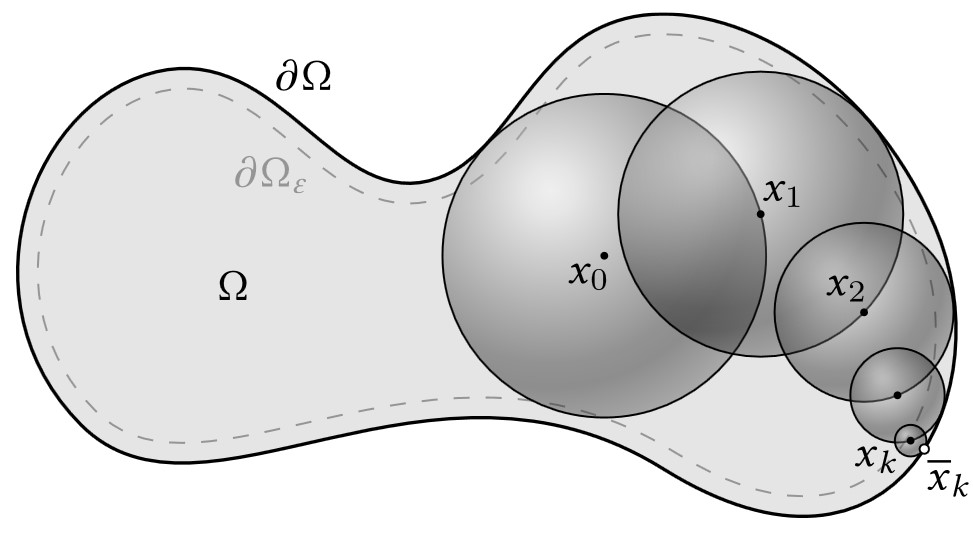
\includegraphics[width=0.6\textwidth]{imgs/Walk_on_Spheres_illustration.jpg}
        \label{fig:Walk_on_Spheres_illustration.jpg}
    \end{figure}
\end{frame}

\section{Monte Carlo}
\begin{frame}
    \frametitle{Monte Carlo}
    \tableofcontentscurrent
\end{frame}

% 2 min
% Als ik aan MC denk, denk ik aan sommen benaderen in het geval
% dat we niet bezitten aan de meeste termen en we veronderstellen
% dat deze tussen 0 en 1 liggen. 

% In het deterministisch geval liggen onze worst case scenarios 
% of van een xi 1 uit elkaar dit beïnvloed onze som 1/k als we
% k-n termen missen dan is onze som enkel afschatten met k-n/k nauwkeurigheid. 
% Als k groot is dan is dit bijna even slecht als geen termen weten.

% De willekeurige oplossing is om de som te samplen of willekeurig termen
% weg laten (wat ik ook Russische roulette noem). Hiervoor krijgen we 
% een vertrouwensinterval via chebychev dat significant kleinder is dan het 
% determinitisch geval het zou zelfs geen probleem zijn als k naar oneindig
% gaat. Dit is de essentie van MC. 

\begin{frame}
    \frametitle{Random sample efficientie van optelling}
    \action<+->{
        Probleem: benader $\bar{x} = \frac{1}{k}\sum_{i=1}^{k} x_{i}$ met $n<<k$ van $x_{i}$'s $\in [0,1]$\\
        (symmetrisch in $x_{i}$) \\
        \vspace{0.2cm}
    }
    \action<+->{
        Vertrouwensinterval kans $=1$  $\sim \frac{k-n}{k}= 1-\frac{n}{k} \approx 1$ \\
        (worst case $\frac{1}{k}$ uit elkaar) \\
        \vspace{0.2cm}
    }
    \action<+->{
        Samplen of termen willekeurig weg laten (Russische roulette)
        \begin{equation}
            \bar{x}  \cong \frac{1}{n}\sum_{i=1}^{n} x_{I_{i}} \cong \frac{1}{k}\sum_{i=1}^{k} B_{i} x_{i}
            .
        \end{equation}
        $\left(E[B_{i}] = 1, P[B_{i}=0]=1-\frac{n}{k}\right)$ \\
        \vspace{0.2cm}
    }
    \action<+->{
        Variantie = RMSE $\sim O\left(\frac{1}{\sqrt{n}}\right)$ en ook vertrouwensintervallen kans $<1$\\
        (CLT of Chebychev's ongelijkheid)\footcitetext{heinrich_optimal_2001}\\
    }

\end{frame}

% 1 min
% Ik heb hier een numeriek voorbeeld bij gestopt
% ik verglijk samplen met en zonder vervanging en
% Russische Roulette. Rechtste plot is het probleem 
% dat ik beschouw en de linkse plot is de convergentie
% van de algoritmes met gemiddeld gezien dezelfde
% hoeveelheid samples en realizaties van de fout 
% ja realizaties want de algoritmes zijn willekeurig. 
% Merk op dat zelfs voor 
% 90% van de samples willekeurige methodes met
% grote kans beter zijn.

\begin{frame}
    \frametitle{Optelling algoritmes (plot)}
    \begin{figure}[h!]
        \centering
        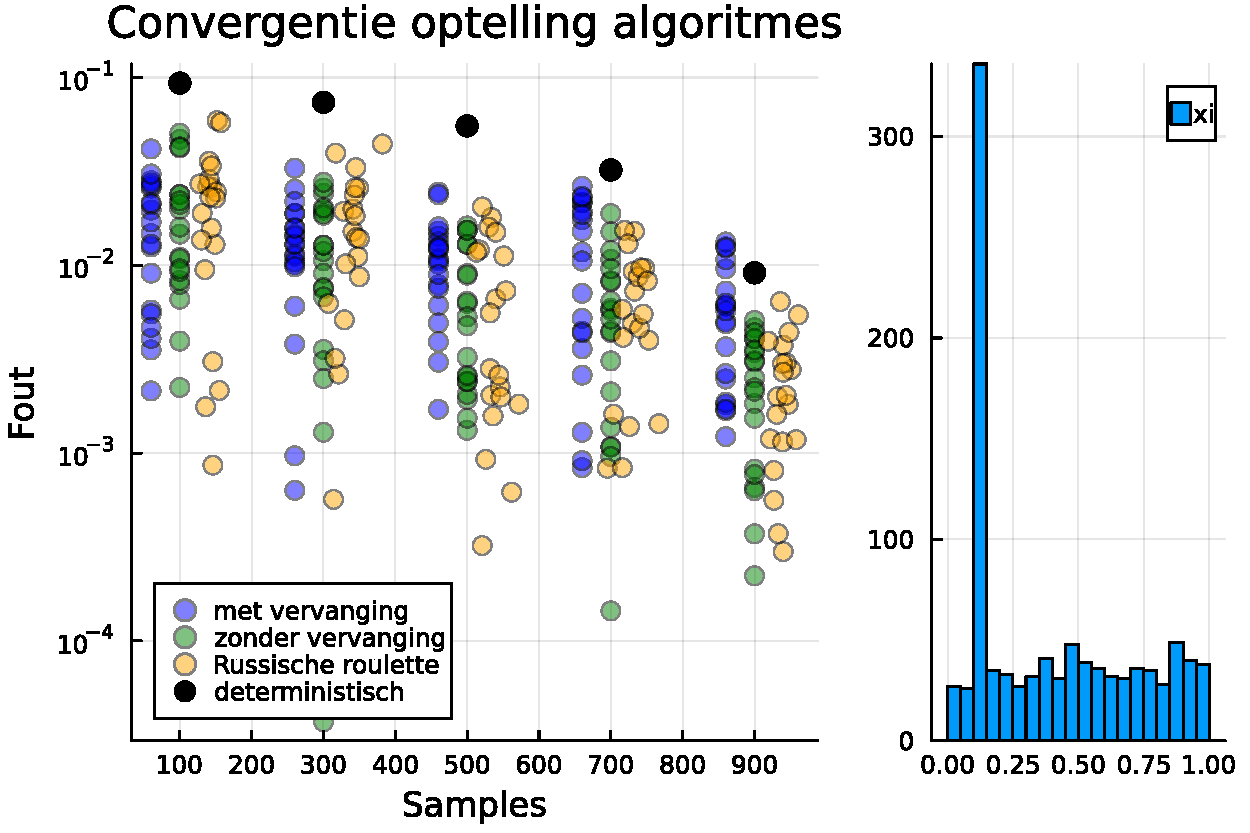
\includegraphics[width=0.8\textwidth]{imgs/convergence_sums.pdf}
        \label{fig:convergentie_optelling}
    \end{figure}
\end{frame}

% 1 min
% integratie is te begrijpen als sommatie
% in de plaats van termen te samplen
% samplen we uniform functie waarden
\begin{frame}
    \frametitle{Monte Carlo integratie}
    Integratie $\approx$ sommatie, integreerbare $f: \mathbb{R} \rightarrow [0,1]$:
    \begin{align}
        \int_{0}^{1} f(s) ds & = E[f(U)]                                 \\
                             & \cong \frac{1}{n} \sum_{j=1}^{n} f(U_{j}) \\
        \text{met } U_{j}    & \sim \text{Uniform}(0,1)
    \end{align}
\end{frame}


\section{Main Poisson algoritme}

% Eindelijk tijd voor het Main Poisson algoritme.
\begin{frame}
    \tableofcontentscurrent
\end{frame}

% 2 min
% Dus neem onze lineaire ODE en veronderstel dat A meetbaar en begrensd is over tijd.
% Merk op dat we hier geen directe veronderstelling maken op y, ik veronderstel
% enkel dat afgeleide zich gedraagt als een afgeleide niet dat ze bestaat.
% Doe beide kanten + sigma y.
% Gebruik de omgekeerde product regel.
% Integreer beide kanten zodat we een integraal vergelijking krijgen.
% Doe een subsitutie, voor de mensen die weten wat importance samplen is we
% importance samplen de exponentiele term, ik herschijf ook de eerste term als
% een integraal.
\begin{frame}
    \frametitle{Main Poisson algoritme}

    \begin{align}
        \action<+->{y_t                              & = A(t) y,  \quad A(t) \text{ meetbaar en } \sup _{t}||A(t)||< \infty  \Leftrightarrow                                                              \\}
        \action<+->{y_t+\sigma y                     & = (\sigma I + A(t)) y \Leftrightarrow                                                                 \\}
        \action<+->{e^{-\sigma t} ( e^{\sigma t}y)_t & = (\sigma I + A(t)) y    \Leftrightarrow                                                               \\}
        \action<+->{y(t)                             & = e^{-\sigma t} y(0) + \int_{0}^{t} e^{(s-t) \sigma} \left(  \left(\sigma I + A(s) \right) y(s)\right) ds,}
    \end{align}
    \action<+->{doe volgende substitutie $e^{(s-t)\sigma} = \tau$, equivalent aan exponentieel te samplen}

    \begin{equation} \label{eq:poisson main}
        \action<+->{
        y(t) = \int_{0}^{e^{-\sigma t}}  y(0) d\tau
        + \int_{e^{-\sigma t}}^{1} \left(  I+ \frac{A(s)}{\sigma} \right)  y(s) d\tau.
        }
    \end{equation}
\end{frame}

% 2min
% Monte Carlo integreer deze integraal,
% de eerste term samplen is geen probleem want we weten y(0)
% maar de tweede term is een probleem want we weten y(s) niet
% we kunnen opnieuw lijn 17 gebruik en recursief Monte Carlo 
% samplen tot we $y(0)$ samplen. Omdat dit een Poisson 
% proces is weet ik hoeveel keer ik moet recursen en 
% kan dit schrijven als een groot product.

\begin{frame}
    \frametitle{Main Poisson algoritme (recursie)}

    \begin{equation} \label{eq:poisson main 2}
        y(t) = \int_{0}^{e^{-\sigma t}}  y(0) d\tau
        + \int_{e^{-\sigma t}}^{1} \left(I+   \frac{A(s)}{\sigma} \right)  y(s) d\tau.
    \end{equation}
    Monte Carlo integreer,  \\
    \action<+->{}
    \action<+->{
        doe dit recursief verder:
        \begin{equation}
            Y(t)= \begin{cases}
                y(0)                                        & \text{als }  e^{-\sigma t} \le  \tau \\
                \left( I+ \frac{A(S)}{\sigma} \right)  Y(S) & \text{anders}
            \end{cases}
            ,
        \end{equation}
        met $S = t +\frac{\ln\left(\tau\right)}{\sigma}$.
    }
    \action<+->{
        \begin{equation}
            y(t) = E \left[ \prod_{k=0}^{N_{t}}\left(I + \frac{A(T_{k})}{\sigma} \right) \right]   y(0).
        \end{equation}
    }
\end{frame}

% We kijken naar een numeriek voorbeeld.
% We nemen A 1 voor t<1/2 and -1 voor t>=1/2
% en dan zijn er 2 manieren waarop het Main Poisson
% algoritme convergeert oftwel door meer simulaties 
% uit te middelen of door sig te verhogen over heel de tijd. Beide 
% hebben een convergentie snelheid van een halve orde 
% wat optimaal is onder de veronderstellingen die we 
% gemaakt hebben. Convergentie in sigma word ook 
% behouden voor nonlineaire problemen.

\begin{frame}
    \frametitle{Main Poisson algoritme (convergentie)}
    \begin{figure}[h!]
        \centering
        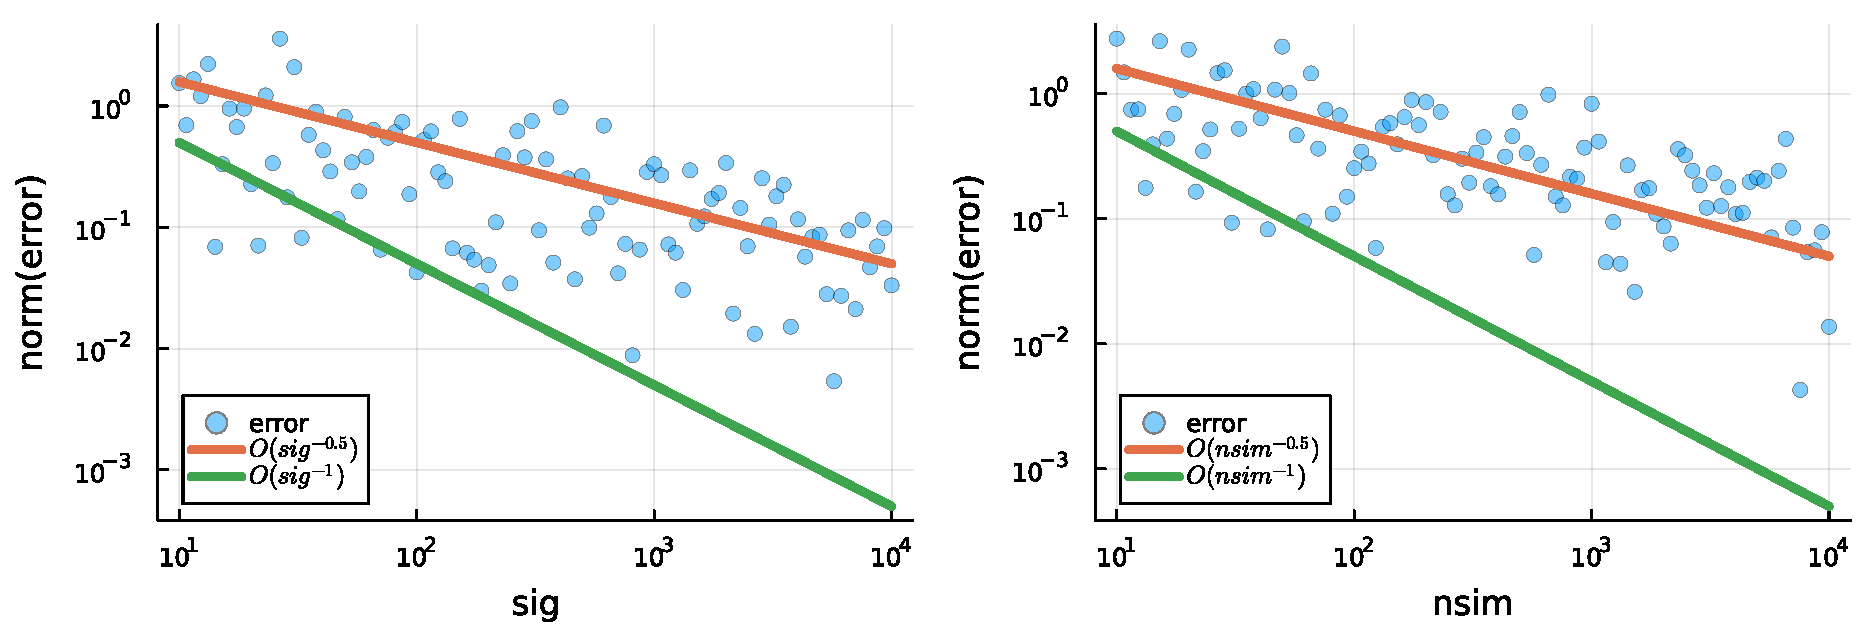
\includegraphics[width=\textwidth]{imgs/convergence_main_poisson.pdf}
        \caption{
            Realisaties $Y(t)$ met $A(t) = \begin{cases}
                    1  & \text{voor } t < 0.5,    \\
                    -1 & \text{voor } t \geq 0.5.
                \end{cases}$ voor verschillende $nsim$ en $sig$.
        }
        \label{fig:imgs/main poisson convergentie}
    \end{figure}
\end{frame}

% We missen de bewijzen dat de verwachtingswaarde en variantie eindig is. Dit is waarschijnlijk
% simpel aan te tonen met de wet van de totale verwachting en variantie.
% We missen ook een bespreking van parallelle complexiteit.
% Ik heb redelijk lang vast gezeten om mijn tijd proces Poison te krijgen ik 
% heb in september dit jaar een paper tegen gekomen van acebron dat dit exact 
% deed voor een specifieke differentiaal vergelijking uiteindelijk als wat ik 
% moest doen was dit veralgemenen.

\begin{frame}
    \frametitle{Main Poisson algoritme (opmerkingen)}
    \begin{equation}
        y(t) \cong Y(t) =  \prod_{k=0}^{N_{t}}\left(I + \frac{A(T_{k})}{\sigma} \right)    y(0).
    \end{equation}
    \begin{itemize}
        \item TB: $E[||Y(t)||],Var[||Y(t)||]< \infty$, wet totale verwachting/variantie
        \item Parallelle complexiteit
        \item Inspiratie uit \cite{acebron_monte_2016}
    \end{itemize}
\end{frame}

\section{Geavanceerde methoden}

\begin{frame}
    \tableofcontentscurrent
\end{frame}

\begin{frame}
    \frametitle{Recursie in Recursie Monte Carlo}
    Next flight uit \cite{sawhney_grid-free_2022}, unbiased methode, $1.5$ orde convergentie,
    moeilijke theorie en te veel functie evaluaties.
    \begin{center}
        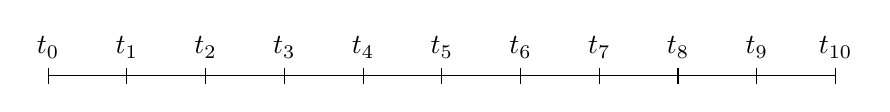
\begin{tikzpicture}
            \draw (0,0) -- (10,0); % horizontal line
            \foreach \x in {0,1,...,10} % loop over labels
            \draw (\x,-0.1) -- (\x,0.1) node[above] {$t_{\x}$}; % draw tick and label
        \end{tikzpicture}
    \end{center}
    \vspace{-0.5cm}
    \begin{align}
        y_{n}          & = \begin{cases}
                               Y_{n-1}(t_{n},y_{n-1}) & \text{ als } n \neq 0        \\
                               y(t_{0})               & \text{ als } n = 0 \nonumber
                           \end{cases} \\
        \\
        Y_{n}(t,y_{n}) & = y_{n} + \Delta t B(t) A(S ) Y_{n}(S,y_{n})
    \end{align}
\end{frame}

\begin{frame}
    \frametitle{Richting Walk on Spheres}
    \setbeamercovered{transparent} % Make uncovered items transparent
    \begin{itemize}
        \item<+->{Plaats discretisatie?}
        \item<+->{Walk on components, $P$ transitie matrix, $Py(0)$ met Monte Carlo}
        \item<+->{Recursieve formulatie $v^{T}y(t)= v^{T}E \left[\prod_{k=0}^{N_{t}}\left(I + \frac{A(T_{k})}{\sigma} \right) \right] y(0) $}
        \item<+->{Recursive first passage sampling}
        \item<+->{Tijdsafhankelijke Russische roulette voor stijve problemen}
        \item<+->{Path stitching vs WoS voor tijd/plaats onafhankelijke problemen}
    \end{itemize}

\end{frame}

\section{Conclusie}

\begin{frame}
    \tableofcontentscurrent
\end{frame}

\begin{frame}
    \frametitle{Conclusie}
    \setbeamercovered{transparent} % Make uncovered items transparent
    \begin{itemize}
        \item<+->{Tevreden met main Poisson algoritme}
        \item<+->{Significante stappen in veralgemenen van WoS}
        \item<+->{Uitgangspunten voor verder onderzoek}
    \end{itemize}

\end{frame}

\begin{frame}[allowframebreaks]{Bibliografie}
    \nocite{daun_randomized_2011,ermakov_monte_2021}
    \printbibliography
\end{frame}

\begin{frame}
    \frametitle{Overzicht integratie}
    Beschouw $f:[0,1]^d \rightarrow [0,1]$ $k$-keer Lipschitz-differentieerbaar:
    \begin{equation}
        \int_{[0,1]^d} f(x) dx  .
    \end{equation}
    CVMC = Control Variate MC, $+0.5$ orde over DET algoritmes \\
    FFT = Clenshaw-Curtis/Gauss Quadrature.
    \begin{table}
        \centering
        \begin{tabular}{lcccc}
                            & $k=-1$ & $0 \le k \le 2$ & $3 \le k \le 5$ & $k>5$ \\
            $d=1$           & MC     & CVMC            & ?               & FFT   \\
            $2 \le d \le 5$ & MC     & CVMC            & CVMC            & ?     \\
            $d>5$           & MC     & MC              & MC              & MC    \\
        \end{tabular}
        \caption{Overzicht integratie algoritmes.}
    \end{table}
\end{frame}

\begin{frame}
    \frametitle{Main Poisson appendix}
    \begin{align}
        y(t) & = E \left[\prod_{k=0}^{N_{t}}\left( I + \frac{A(T_{k})}{\sigma} \right)    \right] y(0)                                             \\
             & = \sum_{n=0}^{\infty}\frac{\sigma^{n} t ^{n}}{n!} E \left[\prod_{k=0}^{n}\left( I + \frac{A(T_{k})}{\sigma} \right)    \right] y(0)
    \end{align}
    Te vergelijken met Magnus expansie.\\
    Voor Monte Carlo transitie matrix hebben we een reductie naar uniformizatie.

\end{frame}

\end{document}
